\section{Frequenzverhalten}

	\subsection{Übertragungsfunktion, Frequenzgang}

		\textbf{Definition} 
		$\underline{F}(\omega) = \dfrac{\underline{X}_a}{\underline{X}_e}$ z.B.$\dfrac{\underline{U}_a}{\underline{U}_e}$\\
		
		\textbf{Bestimmung der UTF}\\
		Um eine möglichst einfache Form der UTF zu erhalten, kann ein simples Vorgehen zur Bestimmung der UTF angewendet werden.
		
		\begin{itemize}
			\item Mit $\underline{U}_a$ beginnen
			\item 1. Strom, welcher durch Element an $\underline{U}_a$ fliesst, mit $\underline{U}_a$ ausdrücken.
			\item 2. Diesen Strom verwenden um Spannung an anderen Elementen auszudrücken.
			\item 3. Mit neuen Spannungen wieder Ströme ausdrücken, usw. Bis $\underline{U}_e$ berechnet ist.
			\item $\Rightarrow$ Wichtig: Jeder Ausdruck darf nur $\underline{U}_a$ und Impedanzen/Admitanzen enthalen. $\Rightarrow$ $\underline{U}_a \cdot (\sum \underline{Z}$)
		\end{itemize} 
		
	\subsection{Frequenznormierung}
		Um den Frequenzgang unabhängig von Werten der Schaltelemente zu machen führt man eine \textbf{normierte Frequenz} $\Omega$ ein.
		
		\begin{tabular}{lllll}
			Normierung &
			$\Omega = \omega/\omega_0 = \omega T$ &
			$\omega_0 = 1/T$ & &
			$\omega_0$ = Bezugsfrequenz\\
			
			Entnormierung &
			$ \omega = \Omega\omega_0 = \Omega / T$ &
			$ T = 1 / \omega_0$ & &
			$\Omega$ = normierte Frequenz 
		\end{tabular}
		
	\subsection{Normierte Netzwerkfunktionen 1.Ordnung}
	\begin{multicols}{2} 
		\subsubsection{Normierte Tiefpassfunktion 1. Ordnung}
		\[ \underline{F} = \dfrac{1}{1 + \im \Omega} \qquad \text{mit} \quad \Omega = \omega T = \omega/\omega_0\]
		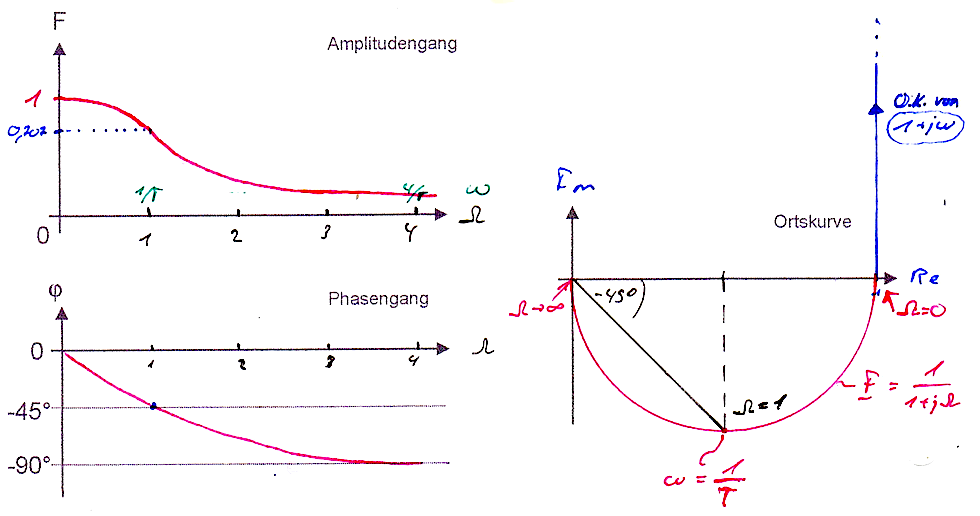
\includegraphics[width=9cm]{./images/freq-norm-TP-1Ordnung}
	\columnbreak
		\subsubsection{Normierte Hochpassfunktion 1. Ordnung}
		\[ \underline{F} = \dfrac{\im \Omega}{1 + \im \Omega} = \dfrac{1}{1 + \frac{1}{\im \Omega}} \qquad \text{mit} \quad \Omega = \omega T = \omega/\omega_0\]
		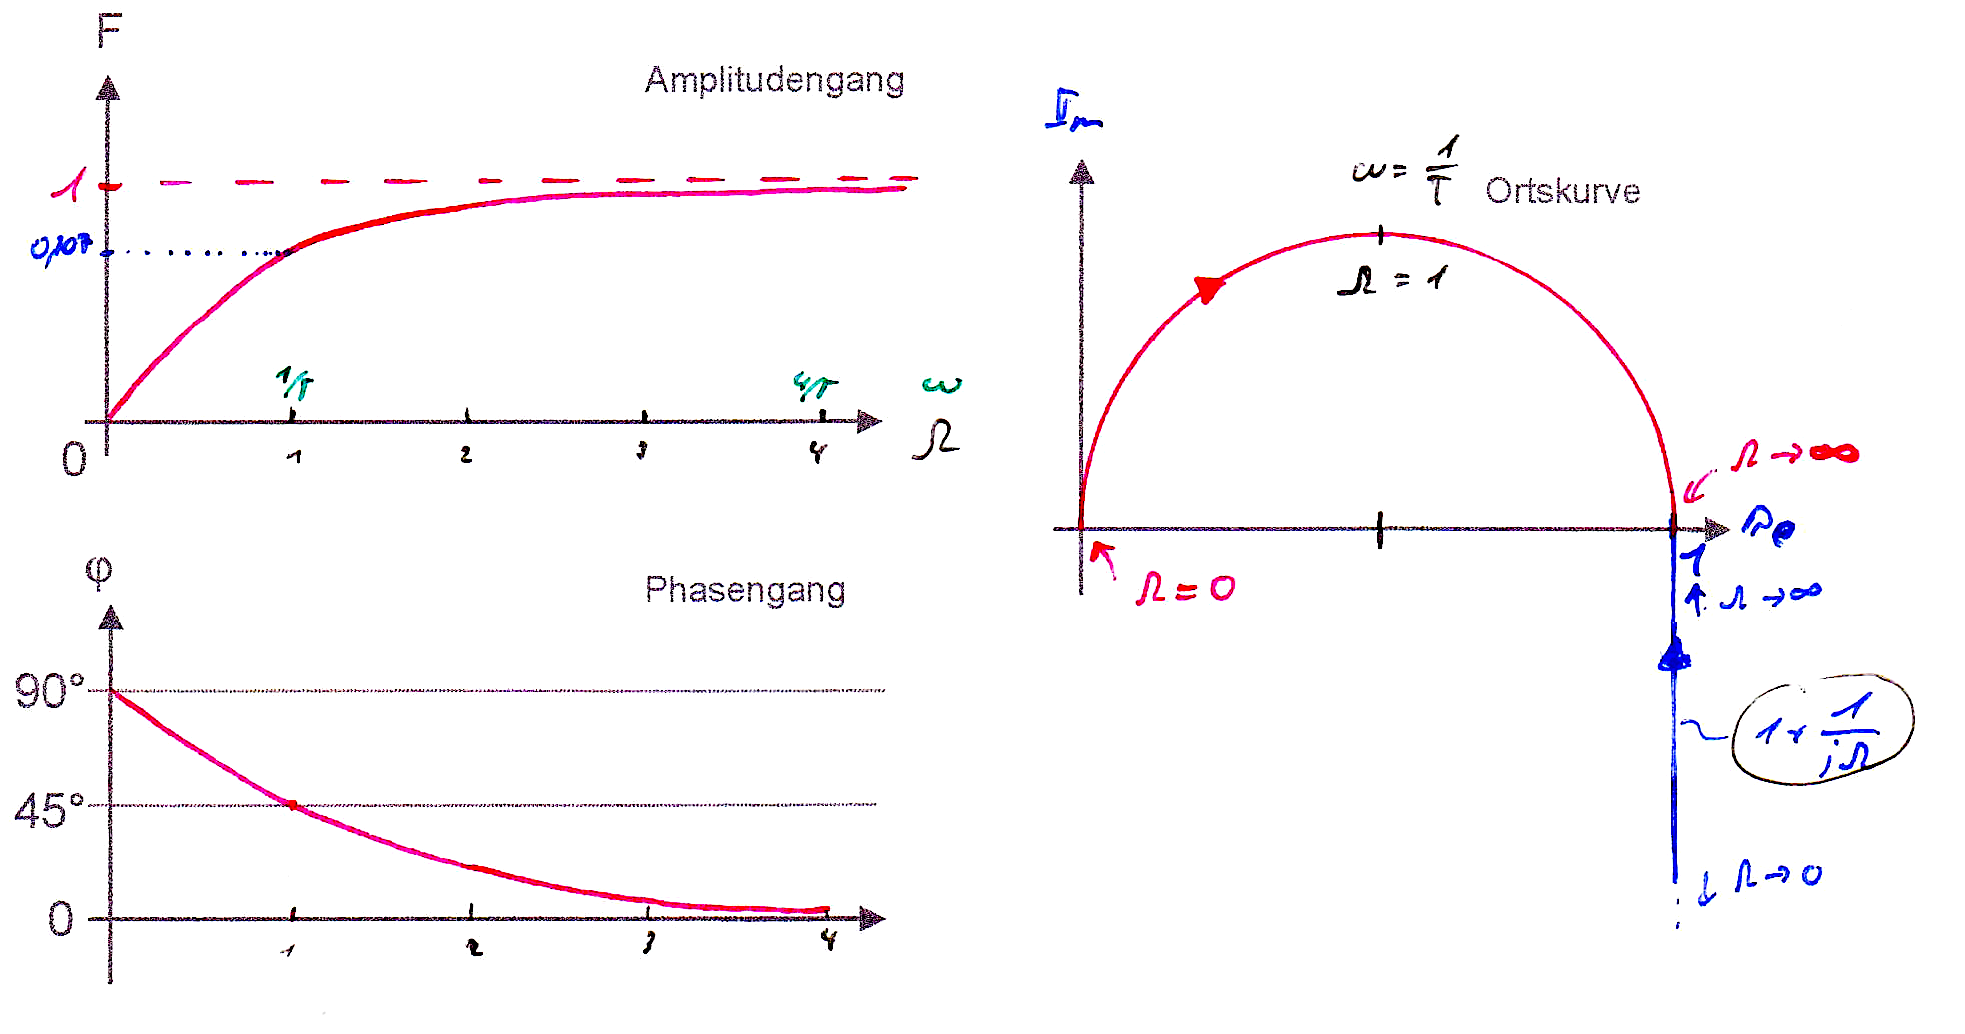
\includegraphics[width=9cm]{./images/freq-norm-HP-1Ordnung}
	\end{multicols}
	
	\subsection{Bodediagramm}
	
	$\boxed{F(\omega)_{dB} = 20 \log F(\omega)} \qquad$
	\textbf{Merke:  } 
	\begin{minipage}{12cm}
		$\underline{F}(\omega) = \underline{F}_1(\omega)\cdot \underline{F}_2(\omega)\cdot \underline{F}_3(\omega) \Rightarrow$
		\parbox{8cm}{Amplitudengang: $ F = F_1\cdot F_2 \cdot F_3$\\
		Phasengang: $\varphi = \varphi_1 + \varphi_2 + \varphi_3$ }\\ \\
		So gilt für den Amplitudengang in dB: 
		$F_{dB}(\omega) = F_{1_{dB}}(\omega) +  F_{2_{dB}}(\omega) + F_{3_{dB}}(\omega)$
	\end{minipage}\\
	
	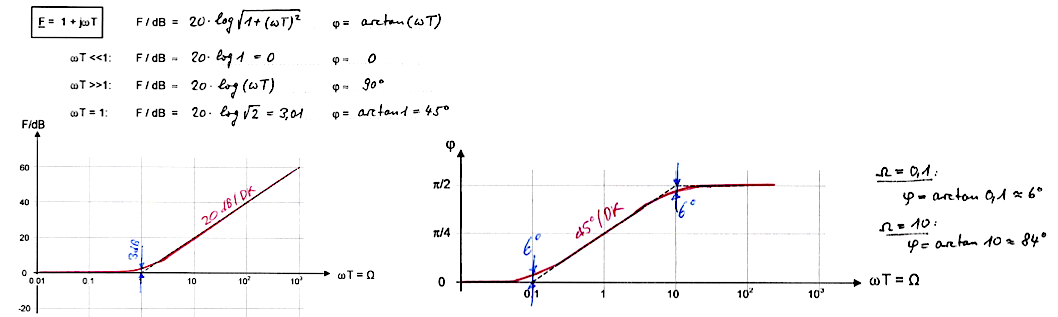
\includegraphics[height = 5cm] {./images/freq-bode-1+jwT}
	
	
	
	

